%%%%%%%%%%%%%%%%%%%%%%%%%%%%%%%%%
%
%       EXERCÍCIO
%
%%%%%%%%%%%%%%%%%%%%%%%%%%%%%%%%%

\definevalorquestao

\begin{exercicioBanco}[\valorquestao]

O histograma representa a distribuição das estaturas de 100 pessoas e as respectivas frequências. Por exemplo, na 3ª classe (\(155\text{--}160\)) estão situadas \(11\%\) das pessoas com estatura de \(1,55\text{ m}\) a \(1,59\text{ m}\). A 5ª classe (\(165\text{--}170\)) chama-se classe mediana. Pelo ponto \(M\) situado na classe mediana, traça-se uma reta paralela ao eixo das frequências, de modo a dividir a área da figura formada pelos nove retângulos das frequências em duas regiões de mesma área. Determine a abscissa do ponto \(M\) (mediana das observações).

\begin{center}
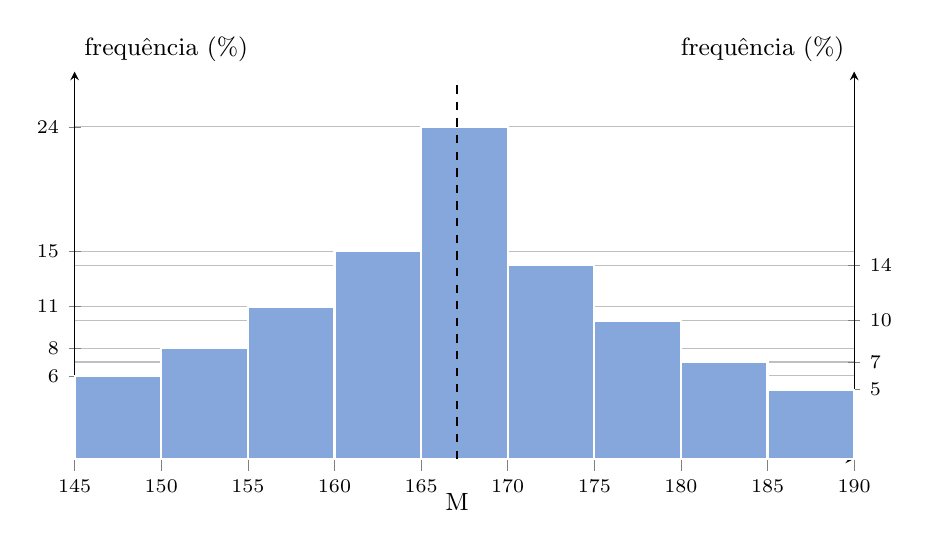
\begin{tikzpicture}
\definecolor{azulAba}{RGB}{133,167,220}

% Eixo Principal (Esquerdo)
\begin{axis}[
    x=0.22cm,
    height=6.5cm,
    ymin=0, ymax=28,
    xmin=145, xmax=190,
    axis lines=left,
    clip=false,
    ytick={6,8,11,15,24},
    xtick={145,150,155,160,165,170,175,180,185,190},
    ylabel={frequência (\%)},
    every axis y label/.style={at={(axis description cs:0,1)},anchor=south west,font=\small},
    y tick label style={font=\scriptsize},
    x tick label style={font=\scriptsize, anchor=north},
    % Controle rigoroso de camadas e linhas horizontais
    set layers,
    ymajorgrids=true,
    grid style={gray!50, thin},
    ybar,
    bar width=1.1cm,
    bar shift=0.55cm,
    enlargelimits=false
]

% Barras azuis opacas (ficam por cima e cobrem as linhas atrás delas)
\addplot[fill=azulAba, draw=white, thick] coordinates {
    (145, 6)
    (150, 8)
    (155, 11)
    (160, 15)
    (165, 24)
    (170, 14)
    (175, 10)
    (180, 7)
    (185, 5)
};

% Linha tracejada da Mediana M e rótulo M
\draw[dashed, black, thick] (axis cs:167.08, 0) -- (axis cs:167.08, 27);
\node[below, font=\small] at (axis cs:167.08, -1.8) {M};

\end{axis}

% Eixo Y Secundário (Direito)
\begin{axis}[
    x=0.22cm,
    height=6.5cm,
    ymin=0, ymax=28,
    xmin=145, xmax=190,
    axis y line=right,
    axis x line=none,
    ytick={5,7,10,14},
    ylabel={frequência (\%)},
    every axis y label/.style={at={(axis description cs:1,1)},anchor=south east,font=\small},
    y tick label style={font=\scriptsize},
    % Linhas horizontais do lado direito
    set layers,
    ymajorgrids=true,
    grid style={gray!50, thin},
    enlargelimits=false
]
\end{axis}
\end{tikzpicture}
\end{center}

\end{exercicioBanco}
